\section{Empirical Evaluation} \label{sec:exp}
In this section, we evaluate our algorithm in comparison
with the state-of-the-art parallelizable algorithms: 
\anm of \shortciteS{Fahrbach2018a} and the algorithm of \shortciteS{Ene2020}.
Also, we compare four versions of our algorithms
with different threshold procedures: \thresam of \shortciteS{Fahrbach2018}, 
two versions of threshold sampling algorithms of \shortciteS{amanatidis2021submodular},
and \threseq proposed in this paper.
Our results are summarized as follows.
~\footnote{Our code is available at 
\textit{https://gitlab.com/luciacyx/nm-adaptive-code.git}.}
\begin{itemize}
\item Our algorithm \latg obtains the best objective
value of any of the parallelizable algorithms;
obtaining an improvement of up to 19\% over the next algorithm,
our \atg. Both \shortciteS{Fahrbach2018a} and \shortciteS{Ene2020} exhibit
a large loss of objective value at both small and large $k$ values; see Figs.
\ref{fig:val-Google} and~\ref{fig:val-Google-largek}.
\item Both our algorithm \atg and \anm use a very small number
of adaptive rounds. Both \latg and the algorithm of \shortciteS{Ene2020}
use roughly an order of magnitude more adaptive rounds; see
Figs.~\ref{fig:rounds-Google} and~\ref{fig:rounds-Google-largek}.
\item The algorithm of \shortciteS{Ene2020} is the most query efficient if access
is provided to an exact oracle 
for the multilinear extension of a submodular function and its gradient
\footnote{The definition of the multilinear extension is given in Appendix~\ref{apx:ene}.};
see Fig.~\ref{fig:query-Google-largek}.
However, if these oracles must be approximated with the set function, 
their algorithm becomes very inefficient and does not scale 
beyond small instances ($n \le 100$); 
see Fig.~\ref{fig:multilinear} in Appendix~\ref{apx:exp}. 
\item Our algorithms used fewer queries to the submodular set function 
than the linear-time algorithm \frg
in \shortciteS{Buchbinder2015a}; see Fig.~\ref{fig:query-Google-largek}.
\item Comparing \atg with four threshold sampling algorithms, 
our \threseq proposed in this paper is the most 
query and round efficient without loss of objective values. 
If running \thresam theoretically, 
with a large amount of sampling in \reducedmean,
the algorithms with \thresam query by a factor of $10^3\sim 10^4$
more than the other algorithms;
see Fig.~\ref{fig:main2}.
\end{itemize}

% that across the three metrics
% of objective value, adapativity, and query complexity,
% \algOnefullname and \anm are very similar, but \algOnefullname
% achieves better objective value on small $k$ values ($k < 200$).
% Over these two algorithms,
% \algTwofullname provides significant improvement in objective value (up to 18\%),
% especially for larger $k$ values ($k = \Omega( n )$), at the cost
% of more adaptive rounds.
% \algTwofullname also outperforms the $\Omega(n \log k)$-adaptive
% algorithm \fig, both in terms of objective value and total number
% of queries. In addition, we show that the state-of-the-art algorithm
% of \cite{Ene2020} for continous, DR-submodular functions 
% does not work well in practice as a heuristic
% for the optimization of discrete set functions. 
% % In summary, both \algOnefullname and \algTwofullname exhibit good
% % objective value, adaptivity, and query complexity. \algOnefullname is more parallelizable
% % at the cost of objective value, especially as $k$ increases. Across all three metrics,
% % the closest competitor is \anm of \cite{Fahrbach2018a}; however, for small $k$ ($k < 200$),
% % the objective value of \anm suffers in comparison to the other algorithms. 

\textbf{Algorithms.}
In addition to the algorithms discussed in the preceding
paragraphs, we evaluate the following baselines:
the \iter algorithm of \shortciteS{Gupta2010a},
and the linear-time $(1/e - \epsi)$-approximation algorithm \frg of \shortciteS{Buchbinder2015a}.
These algorithms are both $O(k)$-adaptive, where $k$ is the cardinality constraint.
%
%the deterministic $1/4$-approximation algorithm \fig of \cite{Kuhnle2019} with query complexity
%and adapativity
%$\Theta (n \log k)$, 

For all algorithms, the accuracy parameter $\epsi$ was set to $0.1$; 
the failure probability $\delta$ was set to 0.1;
$100$ samples
were used to evaluate expectations for \thresam in \anm (thus, this
algorithm was run as heuristics with no performance guarantee). 
Randomized algorithms are averaged over $20$ independent repetitions,
and the mean is reported. The standard deviation is indicated by a shaded
region in the plots. Any algorithm that requires a subroutine for $\unc$
is implemented to use a random set, which is a $(1/4)$-approximation by
\shortciteS{Feige2011}.  

\textbf{Applications.} All combinatorial algorithms are evaluated on two applications
of \sm: the cardinality-constrained maximum cut application and revenue maximization
on social networks, a variant of the influence maximization problem in which $k$ users
are selected to maximize revenue. 
We evaluate on a variety of network technologies from
the Stanford Large Network Dataset Collection \cite{snapnets}.

The algorithm of \shortciteS{Ene2020} requires access to an oracle
for the multilinear extension and its gradient. In the case of maximum cut,
the multilinear extension and its gradient can be computed in closed form
in time linear in the size of the graph, as described in Appendix~\ref{apx:ene}. 
This fact enables us to evaluate
the algorithm of \shortciteS{Ene2020} using direct oracle access to the multilinear
extension and its gradient on the maximum cut application. However,
no closed form exists for the multilinear extension of
the revenue maximization objective. In this case, we found (see Appendix~\ref{apx:exp})
that sampling to approximate the multilinear extension is exorbitant in terms
of runtime; hence, we were unable to evaluate \shortciteS{Ene2020} on revenue maximization.
For more details on the applications and datasets, see
Appendix~\ref{apx:exp}.
\begin{figure*}[t] \centering
  \subfigure[Objective, small $k$]{ \label{fig:val-Google}
    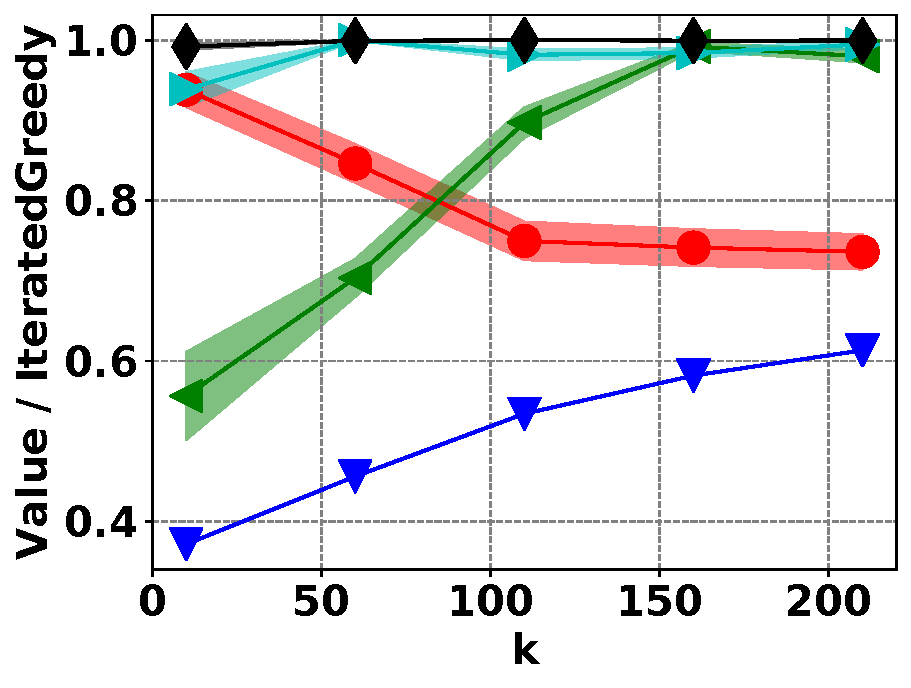
\includegraphics[width=0.3\textwidth,height=0.16\textheight]{plot/google-val-smallK-baseline}
  }
  \subfigure[Rounds, small $k$]{ \label{fig:rounds-Google}
    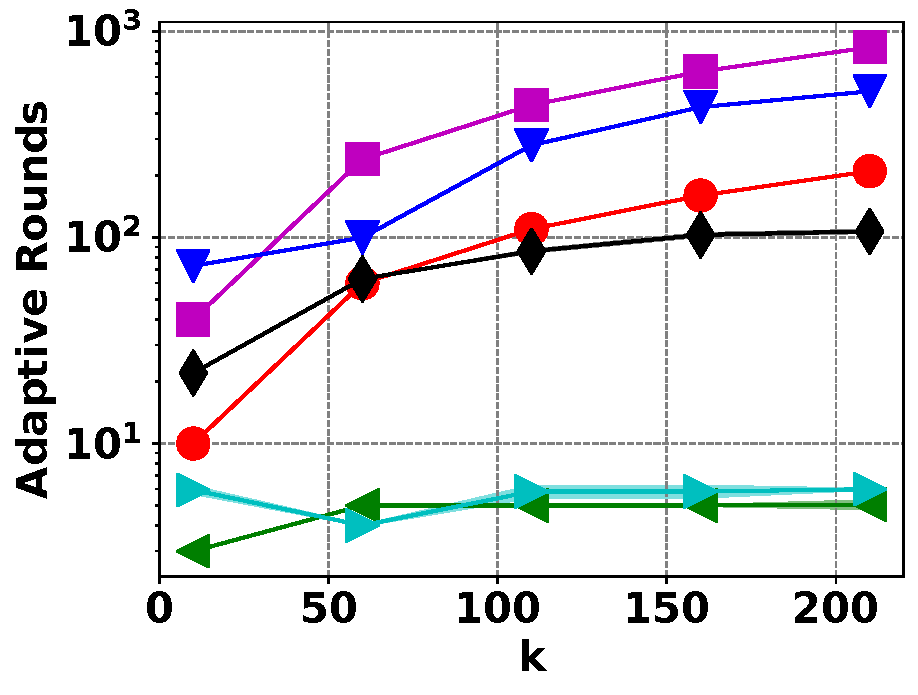
\includegraphics[width=0.3\textwidth,height=0.16\textheight]{plot/google-round-smallK-baseline}
  }
  \subfigure[Legend]{ \label{fig:legend}
  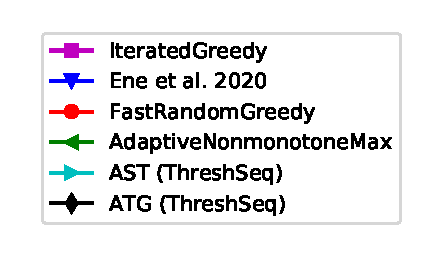
\includegraphics[width=0.3\textwidth,height=0.16\textheight]{plot/legend.pdf}
}
\subfigure[Objective, large $k$]{ \label{fig:val-Google-largek}
  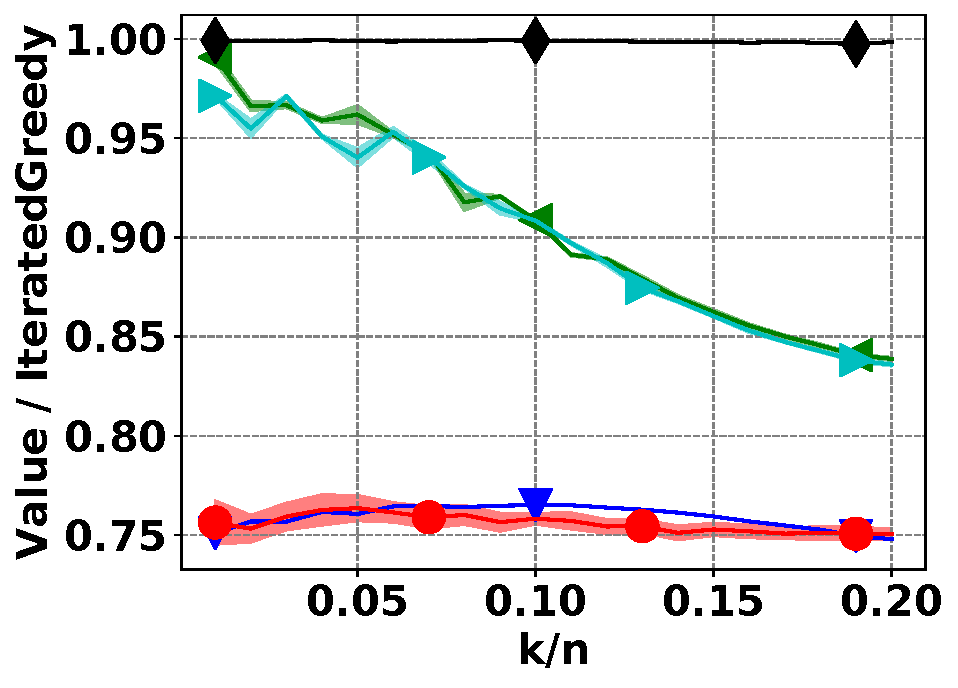
\includegraphics[width=0.3\textwidth,height=0.16\textheight]{plot/google-val-largeK-baseline}
}
\subfigure[Rounds, large $k$]{ \label{fig:rounds-Google-largek}
  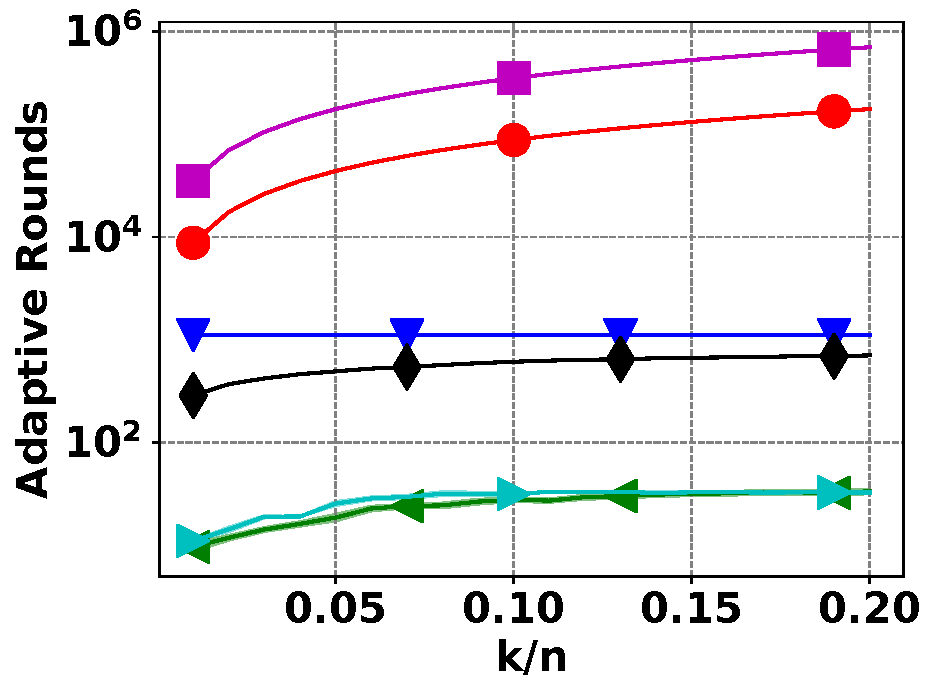
\includegraphics[width=0.3\textwidth,height=0.16\textheight]{plot/google-round-largeK-baseline}
}
  \subfigure[Queries, large $k$]{ \label{fig:query-Google-largek}
    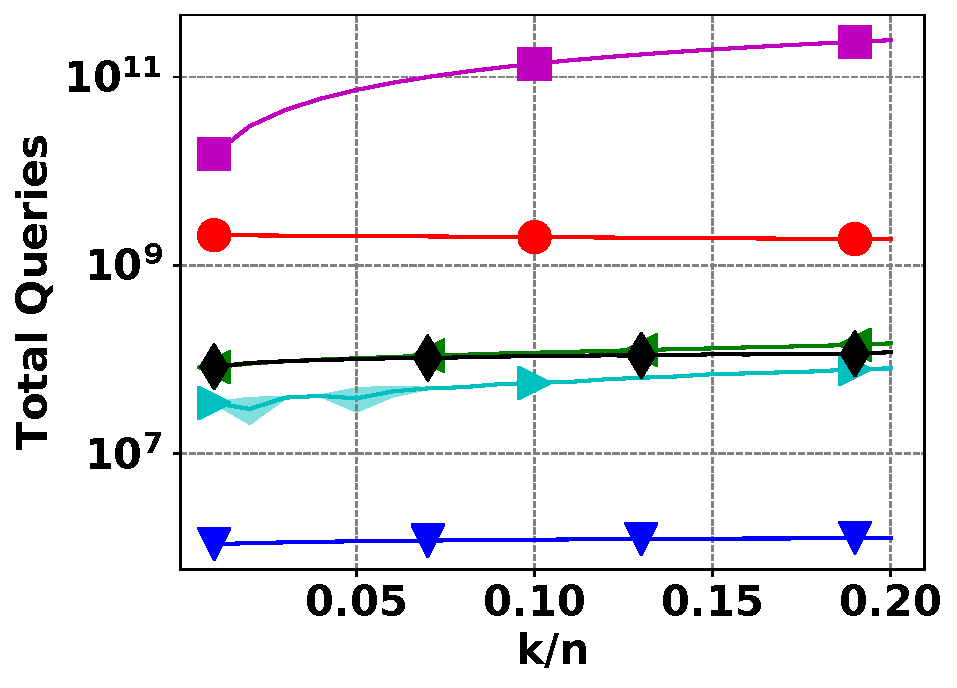
\includegraphics[width=0.3\textwidth,height=0.16\textheight]{plot/google-query-largeK-baseline}
  }
  \caption{Comparison of objective value (normalized by the \iter objective value), 
    total queries, and adaptive rounds on web-Google for the maxcut application for 
    both small and large $k$ values. The large $k$ values are given as a fraction of the number of nodes in the network. The algorithm of \shortciteS{Ene2020} is run with oracle access to the multilinear extension and its gradient; total queries reported for this algorithm are queries to these oracles, rather than the original set function.  } \label{fig:main}
\end{figure*}

\textbf{Results on cardinality-constrained maximum cut.}
In Fig.~\ref{fig:main}, we show representative results for cardinality-constrained
maximum cut on web-Google ($n=875713$)
for both small and large $k$ values. Results on other datasets
and revenue maximization are given in Appendix~\ref{apx:exp}.
In addition, results for \shortciteS{Ene2020} when the multilinear
extension is approximated via sampling are given in Appendix~\ref{apx:exp}.
The algorithms are evaluated by objective value of
solution, total queries made to the oracle, and the number of adaptive rounds (lower is better).
Objective value is normalized by that of \iter. 

In terms of objective value (Figs.~\ref{fig:val-Google} and~\ref{fig:val-Google-largek}), 
our algorithm \latg maintained better than $0.99$ of the \iter value,
while all other algorithms fell below $0.95$ of the \iter value on some instances. 
Our algorithm \atg obtained similar objective value to \anm on larger $k$ values,
but performed much better on small $k$ values. Finally, the algorithm of \shortciteS{Ene2020}
obtained poor objective value for $k \le 100$ and about $0.75$ of the \iter value
on larger $k$ values. It is interesting to observe that the two algorithms with
the best approximation ratio of $1/e$, \shortciteS{Ene2020} and \frg, returned 
the worst objective values on larger $k$ (Fig.~\ref{fig:val-Google-largek}).
% The next
% best was \fig, followed by \atg and \anm, the last of which performed relatively
% poorly
% on $k < 100$. For $k > 100$, \frg achieved the worst objective value, roughly $0.75$ of
% the \iter value. 

For total queries (Fig.~\ref{fig:query-Google-largek}), 
the most efficient is \shortciteS{Ene2020}, although
it does not query the set function directly, but
the multilinear extension and its gradient. The most efficient
of the combinatorial algorithms was 
\atg, followed by \latg.
Finally, with respect to the number of adaptive rounds 
(Fig.~\ref{fig:rounds-Google-largek}), the best was \anm, 
closely followed by \atg; the next lowest was \latg, followed by 
\shortciteS{Ene2020}.
\begin{figure*}[t] \centering
  \subfigure[Objective, BA]{ \label{fig:val-BA-2-ast}
    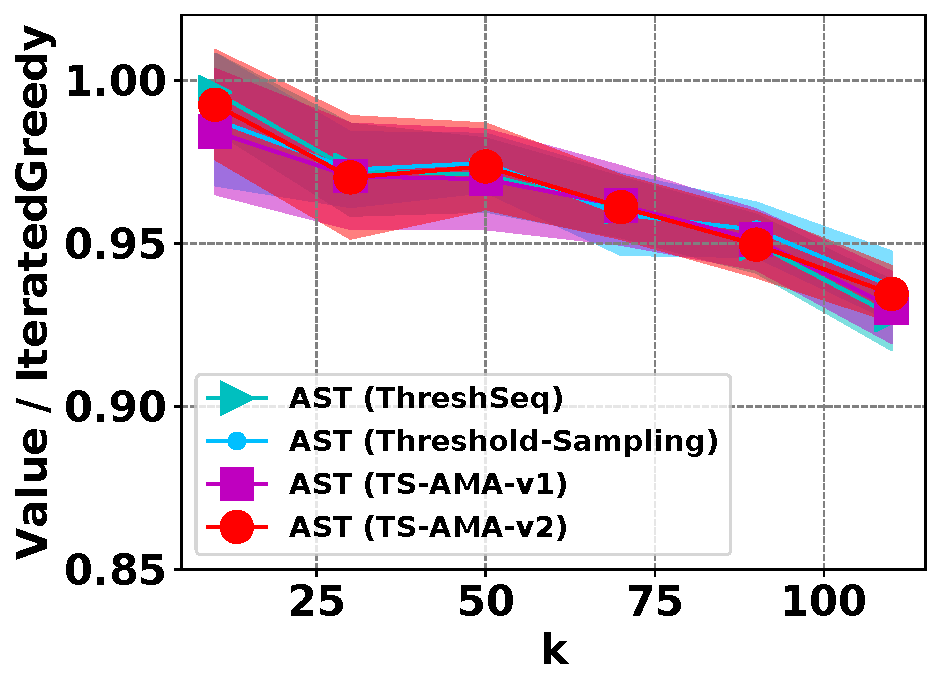
\includegraphics[width=0.3\textwidth,height=0.16\textheight]{plot/BA-val-sample-ast}
  }
  \subfigure[Rounds, BA]{ \label{fig:rounds-BA-2-ast}
    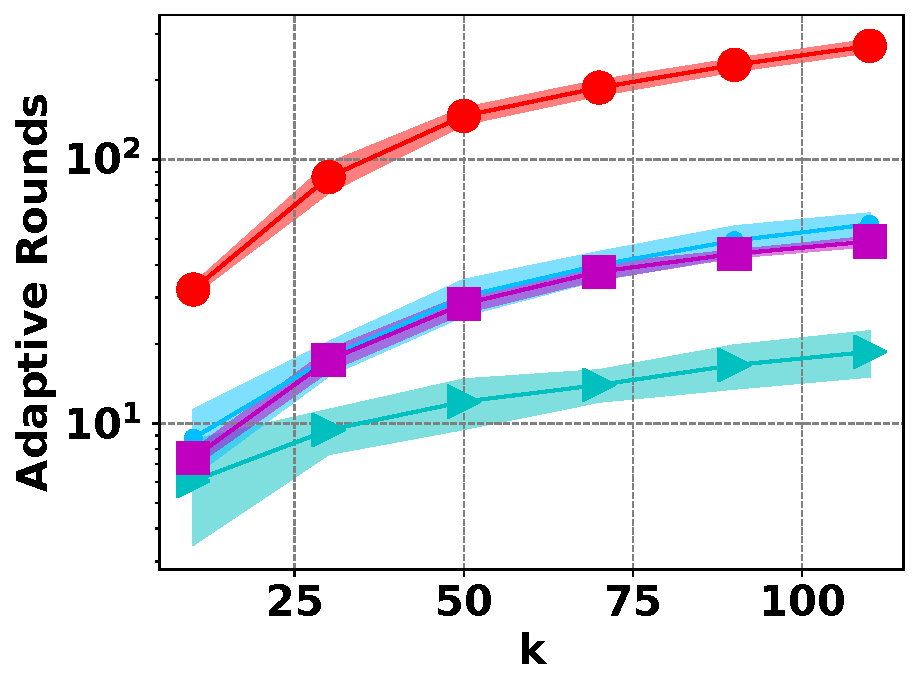
\includegraphics[width=0.3\textwidth,height=0.16\textheight]{plot/BA-round-sample-ast}
  }
  \subfigure[Queries, ca-GrQc]{ \label{fig:query-BA-2-ast}
    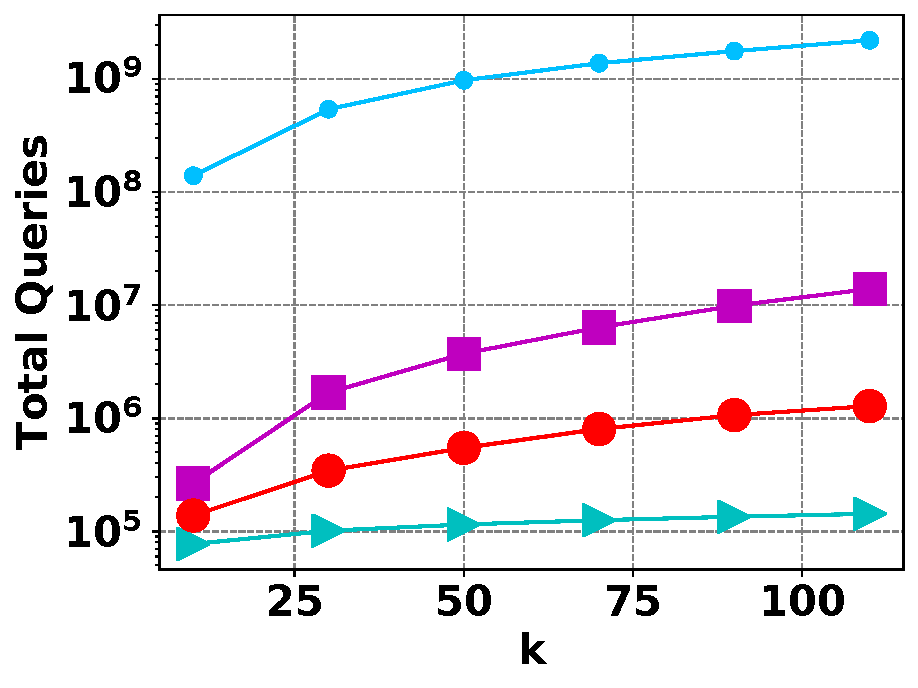
\includegraphics[width=0.3\textwidth,height=0.16\textheight]{plot/BA-query-sample-ast}
  }
  \subfigure[Objective, ca-GrQc]{ \label{fig:val-grqc-2-ast}
    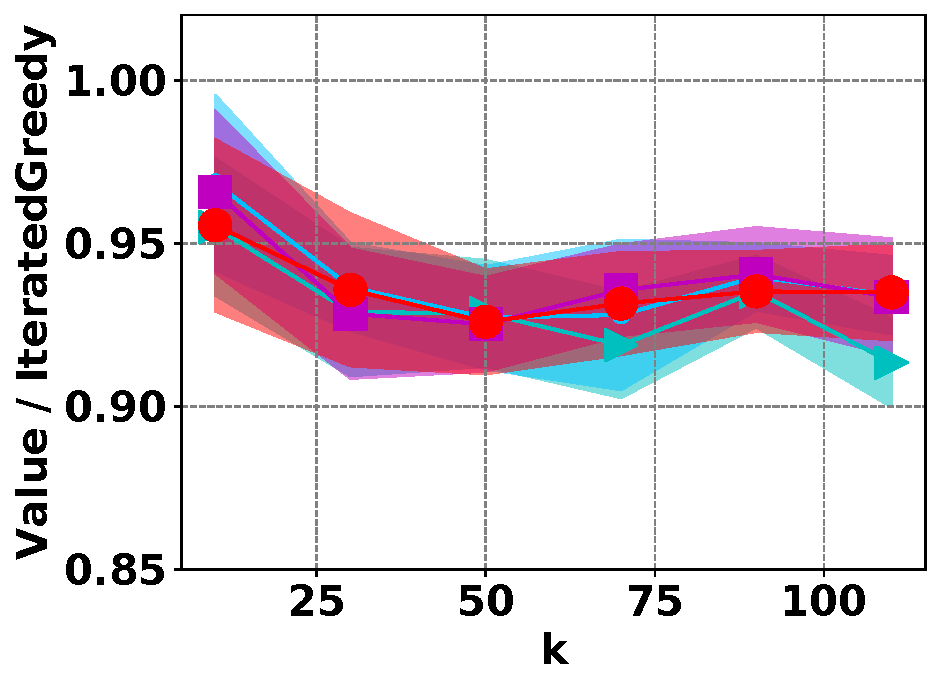
\includegraphics[width=0.3\textwidth,height=0.16\textheight]{plot/grqc-val-sample-ast}
  }
  \subfigure[Rounds, ca-GrQc]{ \label{fig:rounds-grqc-2-ast}
    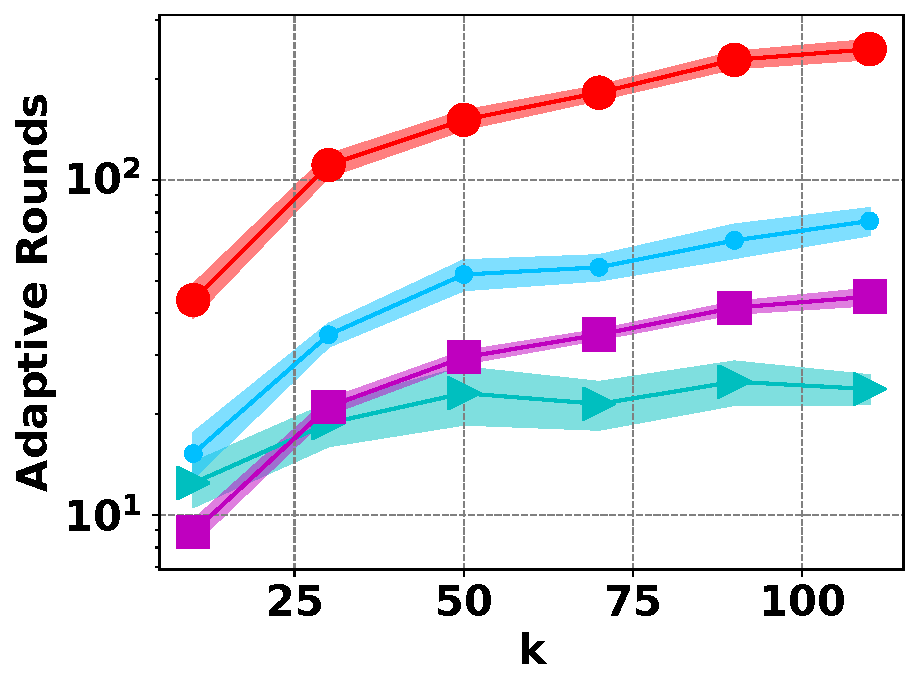
\includegraphics[width=0.3\textwidth,height=0.16\textheight]{plot/grqc-round-sample-ast}
  }
  \subfigure[Queries, ca-GrQc]{ \label{fig:query-grqc-2-ast}
    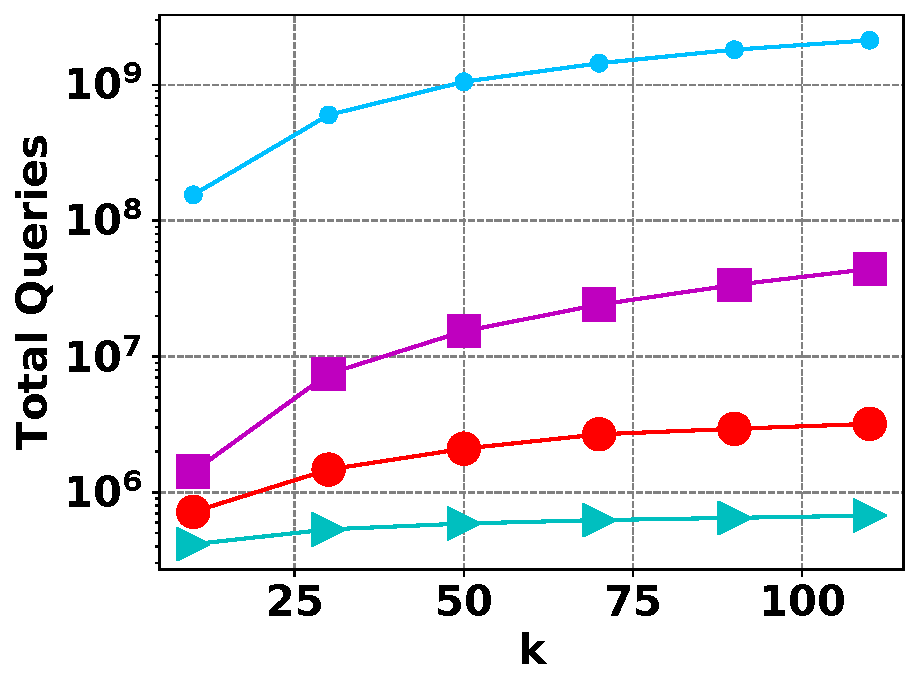
\includegraphics[width=0.3\textwidth,height=0.16\textheight]{plot/grqc-query-sample-ast}
  }
  \caption{Results of \atg with four threshold sampling procedures on two datasets. 
  The algorithms are run strictly following pseudocode.
   } \label{fig:main2}
\end{figure*}

\textbf{Comparison of different threshold sampling procedures.} 
Fig.~\ref{fig:main2} shows the results of \atg 
with different threshold sampling procedures for cardinality-constrained maximum cut 
on two datasets, BA ($n=968$) and ca-GrQc ($n = 5242$).
All the algorithms are run according to pseudocode without any modification.
\threseqama and \tsbin represent the \threseq algorithms without and with
binary search proposed in \shortciteS{amanatidis2021submodular}.

For objective values, all four versions of \atg return similar results;
see Figs.~\ref{fig:val-BA-2-ast} and~\ref{fig:val-grqc-2-ast}.
As for adaptive rounds, \threseq, \thresam, and \threseqama all run in
$\oh{\log(n)}$ rounds, while \tsbin runs in $\oh{\log^2(n)}$ rounds.
By the results in Figs.~\ref{fig:rounds-BA-2-ast} and~\ref{fig:rounds-grqc-2-ast},
our \threseq is the most highly parallelizable algorithm, followed by \threseqama.
\tsbin is significantly worst as what it is in theory.
With respect to the query calls,
while our \threseq only queries once for each prefix,
\thresam queries $16\lceil \log(2/\hat{\delta})/\hat{\epsi}^2 \rceil$ times,
and both \threseqama and \tsbin query $|V|$ times.
According to Figs.~\ref{fig:query-BA-2-ast} and~\ref{fig:query-grqc-2-ast},
our \threseq is the most query efficient one among all.
Also, the total queries do not increase a lot when $k$ increases.
With binary search, \tsbin is the second best one which has $\oh{n\log^2(n)}$
query complexity.
As for \thresam,
with the input values as $n=968$, $k=10$, and $\epsi = \delta = 0.1$,
it queries about $2\times 10^5$ times for each prefix
which is significantly large.

Among all, \threseq proposed in this paper is not only the best theoretically,
but also performs well in experiments compared with
the pre-existing threshold sampling algorithms.

% As for the two variants of \threseq proposed 
% in \cite{amanatidis2021submodular}.
% Algorithms with \threseqama save the rounds but induce more queries,
% while \tsbin saves the queries but increases the rounds.

% In regard to objective value, all different versions of \atg get similar 
% objective values. So do \latg.
% With respect to adaptive rounds, all the threshold procedures
% runs within $\oh{\log(n)}$ rounds except the \tsbin 
% which runs within $\oh{\log(n)\log(k)}$ rounds.
% From Fig.~\ref{fig:rounds-BA-2} and ~\ref{fig:rounds-grqc-2}, 
% \atg with \threseq proposed in this paper is the most efficient.
% The adaptive rounds of \atg(\tsbin) increases apparently
% compared with other \atg algorithms.
% Also, since each iteration of \latg calls a threshold subroutine
% which is based on the previous iterations and 
% a slowly decreasing threshold $\tau$,
% after first filtration, the size of candidate set is limited.
% Thus, there is no significant difference between different \latg.

% As for number of queries, from Fig.~\ref{fig:query-grqc-2}, 
% \atg with \threseq proposed in this paper is still the most query efficient.
% Next, we discuss the results of all algorihtms except ones with \thresam.
% Since the query complexity of \threseqama is $\oh{n^2\log(n)}$,
% \atg(\threseqama) queries more than \atg with \threseq and \tsbin.

%%% Local Variables:
%%% mode: latex
%%% TeX-master: "main"
%%% End:
